\section{第4章\quad Smith圆图与阻抗匹配}
\begin{frame}{第4章\quad Smith圆图与阻抗匹配}
  上世纪六十年代以来,在微波工程和微波技术上,出现了一次不小的革命,即所谓MIC(Microwave Integrated Circuit)微波集成电路——HMIC、MMIC。其特色是体积小、功能多、频带宽,但承受功率小。因此被广泛应用于接收机和小功率元件中,并都传输TEM波。\\
  作为这一革命的“过渡人物”是带状线(Stripline)。它可以看作是同轴线的变形。
\end{frame}

\subsection{Smith圆图}
\begin{frame}{Smith圆图}
  前面的分析都是围绕如下公式及相互关系展开的:
  \begin{empheq}[box=\widefbox]{align*}
   Z_{in}(d)=\frac{V_L\cosh\gamma d+I_LZ_0\sinh\gamma d}{I_L\cosh\gamma d+\frac{V_L\sinh\gamma d}{Z_0}} & =Z_0\frac{Z_L+Z_0\tanh\gamma d}{Z_0+Z_L\tanh\gamma d}\\
   \text{无耗传输线:}& =Z_0\frac{Z_L+jZ_0\tan\beta d}{Z_0+jZ_L\tan\beta d}
  \end{empheq}
  \begin{columns}
   \begin{column}{0.45\linewidth}
    \begin{empheq}[box=\widefbox]{align*}
     \Gamma_L &=\frac{A_2}{A_1}=\frac{Z_L-Z_0}{Z_L+Z_0}\\
     &=\left\lvert\frac{Z_L-Z_0}{Z_L+Z_0}\right\rvert e^{j\phi_L}\\
     &=\lvert\Gamma_L\rvert e^{j\phi_L}
    \end{empheq}
   \end{column}
   \begin{column}{0.55\linewidth}
    \begin{empheq}[box=\widefbox]{align*}
     \rho=VSWR=\frac{\lvert V\rvert_{max}}{\lvert V\rvert_{min}}=\frac{1+\lvert\Gamma_L\rvert}{1-\lvert\Gamma_L\rvert}
    \end{empheq}
   \end{column}
  \end{columns}
\end{frame}

\begin{frame}{Smith Chart(阻抗圆图及其应用)}
  \begin{enumerate}
   \item 圆图概念
         \begin{itemize}
          \item 圆图是求解均匀传输线有关阻抗计算和阻抗匹配问题的一类曲线坐标图;
          \item 图上有两组坐标曲线:归一化阻抗或者导纳的实部和虚部的等值线簇,与反射系数的模和辐角的等值线簇;
          \item 所有这些等值线簇都是圆或圆弧(直线是圆的特例),故称为阻抗圆图或者导纳圆图,简称圆图。
         \end{itemize}
         \saveenum
  \end{enumerate}
  \begin{align*}
   z(d)=\frac{Z(d)}{Z_0}=\frac{1+\Gamma(d)}{1-\Gamma(d)}\quad\text{or}\quad\Gamma(d)=\frac{z(d)-1}{z(d)+1} \\
   z(d)=r(d)+jx(d)=\lvert z\rvert e^{j\theta}                                                              \\
   \Gamma(d)=\Gamma_{Re}(d)=j\Gamma_{Im}(d)=\lvert\Gamma(d)\rvert e^{j\phi(d)}
  \end{align*}
 \end{frame}
 
 \begin{frame}{Smith Chart(阻抗圆图及其应用)}
  \begin{enumerate}
   \resume
   \item Smith圆图
         \begin{itemize}
          \item Smith圆图是通过双线性变换式,将$z$复平面上的$r=$常数和$x=$常数的二簇相互正交的直线分别变换成$\Gamma$复平面上的二簇相互正交的圆,并同$\Gamma$极坐标等值线簇$\lvert\Gamma\rvert=$常数和$\phi=$常数套印在一起而得到的圆图。
          \item 该图表是由\textbf{Phillip Smith}于1939年发明的,当时他在美国的RCA公司工作。Smith也许不是图表的第一位发明者,一位名叫Kurakawa的日本工程师声称早于其一年发明了这种图表。
         \end{itemize}
  \end{enumerate}
  \begin{align*}
   z(d)=\frac{Z(d)}{Z_0}=\frac{1+\Gamma(d)}{1-\Gamma(d)}\quad\text{or}\quad\Gamma(d)=\frac{z(d)-1}{z(d)+1} \\
   z(d)=r(d)+jx(d)=\lvert z\rvert e^{j\theta}                                                              \\
   \Gamma(d)=\Gamma_{Re}(d)=j\Gamma_{Im}(d)=\lvert\Gamma(d)\rvert e^{j\phi(d)}
  \end{align*}
 \end{frame}
 
 \begin{frame}{Smith Chart(阻抗圆图及其应用)}
  \begin{itemize}
   \item 阻抗圆图\\
         阻抗圆图是由等反射系数圆和归一化等阻抗圆组成。
         \begin{enumerate}
          \item 等反射系数圆\\
                距离终端$d$处的反射系数为
                \begin{empheq}[box=\widefbox]{align*}
                 \Gamma(d)=\lvert\Gamma\rvert e^{j\phi(d)}=\lvert\Gamma_L\rvert e^{j(\phi_L-2\beta d)}=\Gamma_{Re}+j\Gamma_{Im}
                \end{empheq}
                \saveenum
         \end{enumerate}
  \end{itemize}
  表明,在复平面上等反射系数模$\lvert\Gamma\rvert$的轨迹是以坐标原点为圆心、$\lvert\Gamma_L\rvert$为半径的圆,这个圆称为等反射系数$\lvert\Gamma\rvert$圆。由于反射系数的模与驻波比是一一对应的,故又称为\textbf{等驻波比圆}。
 \end{frame}
 
 \begin{frame}{Smith Chart(阻抗圆图及其应用)}
  线上移动的距离与转动角度之间的关系为
  \begin{columns}
   \begin{column}{0.4\linewidth}
    \begin{empheq}[box=\widefbox]{align*}
     \Gamma(d) &=\lvert\Gamma\rvert e^{j\phi}\\
     &=\lvert\Gamma_L\rvert e^{j(\phi_L-2\beta d)}\\
     \Delta\phi &=2\beta\Delta d\\
     &=\frac{4\pi}{\lambda}\Delta d
    \end{empheq}
    为了使用方便,有的圆图上标有两个方向的波长数数值,如图所示。向负载方向移动读里圈读数,向波源方向移动读外圈读数。
   \end{column}
   \begin{column}{0.6\linewidth}
    \begin{figure}
     \includegraphics[width=6cm]{reflect_coeff.png}
     \caption{反射系数圆}
    \end{figure}
   \end{column}
  \end{columns}
 \end{frame}
 
\begin{frame}{Smith Chart(阻抗圆图及其应用)}
  \begin{tikzpicture}
    \begin{smithchart}
      \coordinate [label=below:$O$] (a) at (0pt,0pt);
      \coordinate [label=above:$2+\mathrm{j}1$] (b) at (2,1);
      %\path [draw=blue] (H) circle (2.83cm);
      %\path[draw=red] (a) circle (2.83cm);
      \node [draw=red] at (a) [circle through={(b)}] {};
      %\path[draw=blue] (0.2,0.5) circle (0.75cm);
      \path[draw=blue,fill=blue] (b) circle (0.05cm);
      %\path[draw=blue] (a) -- (2,1);
      \draw (a) -- ($ (a) !2.3! (b) $) coordinate (c);
    \end{smithchart}

    \node at (c) [anchor=south] {$0.213\lambda$}; 
  \end{tikzpicture}
  
  %\begin{tikzpicture}
  %  \draw[help lines] (0,0) grid (3,2);
  %  \node (a) at (2,1.5) {$a$};
  %  \node [draw] at (1,1) [circle through={(a)}] {$c$};
  %\end{tikzpicture}

\end{frame}

\begin{frame}
  \begin{tikzpicture}
    \begin{smithchart}
      % Reactance plot
      \addplot[domain=0:90,samples=600,color=blue]{.5};
      % Resistance plot - orange
      \addplot+[mark=*,only marks,samples at={.5,.51,...,5},
      mark options={solid},color={orange},mark size=.2,line width=1](.5,x);
      % Resistance plot - red
      \addplot+[mark=*,only marks,samples at={0,.01,...,.5},
      mark options={solid},color={red},mark size=.2,line width=1](1,x);
    \end{smithchart}
  \end{tikzpicture}
\end{frame}



 \begin{frame}{Smith Chart(阻抗圆图及其应用)}
  \textbf{相角相等的反射系数的轨迹是单位圆内的径向线}
  \begin{columns}
   \begin{column}{0.4\linewidth}
    线上移动长度$\lambda/2$时,对应反射系数矢量转动一周。一般转动的角度用波长数(或电长度)$\Delta d/\lambda$表示,且标度波长数的零点位置通常选在$\phi=\pi$处。
   \end{column}
   \begin{column}{0.6\linewidth}
    \begin{figure}
     \includegraphics[width=4cm]{reflect_coeff.png}
     \caption{等反射系数圆的波长数标度}
    \end{figure}
   \end{column}
  \end{columns}
  $\phi=0$\textbf{的径向线为各种不同负载阻抗情况下电压波腹点反射系数的轨迹;}\\
  $\phi=\pi$\textbf{的径向线为各种不同负载阻抗情况下电压波节点反射系数的轨迹。}
 \end{frame}
 
 \begin{frame}{Smith Chart(阻抗圆图及其应用)}
  \begin{itemize}
   \item 阻抗圆图
         \begin{enumerate}
          \resume
          \item 归一化阻抗圆
         \end{enumerate}
         \begin{empheq}[box=\widefbox]{align*}
          z_{in}(d)=\frac{Z_{in}(d)}{Z_0}=\frac{1+\Gamma(d)}{1-\Gamma(d)}
         \end{empheq}
  \end{itemize}
  \begin{align*}
   z_{in}(d) & =\frac{1+(\Gamma_{Re}+j\Gamma_{Im})}{1-(\Gamma_{Re}+j\Gamma_{Im})}                                                                          \\
             & =\frac{1-(\Gamma^{2}_{Re}+\Gamma^{2}_{Im})}{(1-\Gamma_{Re})^2+\Gamma_{Im}^{2}}+j\frac{2\Gamma_{Im}}{(1-\Gamma_{Re})^2+\Gamma_{Im}^{2}}=r+jx
  \end{align*}
  \begin{empheq}[box=\widefbox]{align*}
   \left(\Gamma_{Re}-\frac{r}{r+1}\right)^2+\Gamma_{Im}^{2}=\frac{1}{(r+1)^2}\quad \text{归一化电阻轨迹方程}\\
   (\Gamma_{Re}-1)^2+\left(\Gamma_{Im}-\frac{1}{x}\right)^2=\left(\frac{1}{x}\right)^2\quad \text{归一化电抗轨迹方程}
  \end{empheq}
  \footnotesize{特征参数,是形成统一Smith圆图的最关键点,它包含了阻抗归一和电长度归一。}
 \end{frame}
 
 \begin{frame}{Smith Chart(阻抗圆图及其应用)}
   \only<1>{\begin{columns}
     \begin{column}{0.55\linewidth}
       \begin{empheq}[box=\widefbox]{align*}
         (\Gamma_{Re}-1)^2+\left(\Gamma_{Im}-\frac{1}{x}\right)^2=\left(\frac{1}{x}\right)^2
       \end{empheq}
     \end{column}
     \begin{column}{0.45\linewidth}
       \begin{figure}
         \includegraphics[width=5cm]{diankangyuan.png}
         \caption{归一化电抗圆}
       \end{figure}
     \end{column}
   \end{columns}}
   \only<2>{\begin{columns}
     \begin{column}{0.45\linewidth}
       \begin{figure}
         \includegraphics[width=5cm]{dianzuyuan.png}
         \caption{归一化电阻圆}
       \end{figure}
     \end{column}
     \begin{column}{0.55\linewidth}
       \begin{empheq}[box=\widefbox]{align*}
         \left(\Gamma_{Re}-\frac{r}{r+1}\right)^2+\Gamma_{Im}^2=\frac{1}{(r+1)^2}
       \end{empheq}
     \end{column}
   \end{columns}}
 \end{frame}
 
 \begin{frame}{Smith Chart(阻抗圆图及其应用)}
   电阻圆始终和直线$\Gamma_r=1$相切
   \begin{columns}
     \begin{column}{0.42\linewidth}
       \begin{figure}
         \includegraphics[width=4.55cm]{dianzuyuan.png}
         \caption{归一化电阻圆}
       \end{figure}
     \end{column}
     \begin{column}{0.58\linewidth}
       \begin{tabular}{|c|c|c|c|}
         \hline
         \multirow{2}*{$r$} &
         \multicolumn{2}{c|}{\footnotesize{圆心坐标}} &
         \multirow{2}*{\footnotesize{半径} $\left(\frac{1}{1+r}\right)$}\\ \cline{2-3}
         & $\Gamma_r=\frac{r}{1+r}$ & $\Gamma_i=0$ \\ \hline
         0 & 0 & 0 & 1 \\ \hline
         1 & 1/2 & 0 & 1/2 \\ \hline
         2 & 2/3 & 0 & 1/3 \\ \hline
       \end{tabular}
     \end{column}
   \end{columns}
   \begin{empheq}[box=\widefbox]{align*}
     \left(\Gamma_{Re}-\frac{r}{r+1}\right)^2+\Gamma_{Im}^2=\frac{1}{(r+1)^2}
   \end{empheq}
 \end{frame}
 
 \begin{frame}{Smith Chart(阻抗圆图及其应用)}
   电抗圆圆心坐标和半径
   \begin{empheq}[box=\widefbox]{align*}
       (\Gamma_{Re}-1)^2+\left(\Gamma_{Im}-\frac{1}{x}\right)^2=\left(\frac{1}{x}\right)^2
   \end{empheq}
   \begin{columns}
     \begin{column}{0.58\linewidth}
       \begin{tabular}{|c|c|c|c|}
         \hline
         \multirow{2}*{$x$} &
         \multicolumn{2}{c|}{\footnotesize{圆心坐标}} &
         \multirow{2}*{\footnotesize{半径} $\left(\frac{1}{x}\right)$}\\ \cline{2-3}
         & $\Gamma_r=1$ & $\Gamma_i=\frac{1}{x}$ \\ \hline
         0 & 1 & \infty & \infty \\ \hline
         \pm0.5 & 1 & \pm2 & 2 \\ \hline
         \pm1 & 1 & \pm1 & 1 \\ \hline
       \end{tabular}
     \end{column}
     \begin{column}{0.42\linewidth}
       \begin{figure}
         \includegraphics[width=4.55cm]{diankangyuan.png}
         \caption{归一化电抗圆}
       \end{figure}
     \end{column}
   \end{columns}
 \end{frame}
 
 \begin{frame}{Smith Chart(阻抗圆图及其应用)}
   将等电阻圆和等电抗圆绘制在同一张图上,得到阻抗圆图。
   \centering
   \includegraphics[width=8cm]{zukangyuan.png}
 \end{frame}
 
 \begin{frame}{Smith Chart(阻抗圆图及其应用)}
   阻抗圆图有如下几个特点
   \begin{columns}
     \begin{column}{0.4\linewidth}
       (1)圆图上有三个特殊点:\\
       \pause\textbf{匹配点}(O点),其坐标为(0,0)\\
       $r=1,x=0$ \\
       $\lvert\Gamma\rvert=0,\rho=1$\\
       \pause\textbf{短路点}(C点),其坐标为(-1,0)\\
       $r=0,x=0,\lvert\Gamma\rvert=1$ \\
       $\rho=\infty,\phi=\pi$ \\
       \pause\textbf{开路点}(D点),其坐标为(1,0)\\
       $r=\infty,x=\infty,\lvert\Gamma\rvert=1$ \\
       $\rho=\infty,\phi=0$
     \end{column}
     \begin{column}{0.6\linewidth}
       \only<1>{\includegraphics[width=5cm]{smithchart-1.png}}
       \only<2>{\includegraphics[width=5cm]{smithchart-2.png}}
       \only<3>{\includegraphics[width=5cm]{smithchart-3.png}}
     \end{column}
   \end{columns}
 \end{frame}
 
 \begin{frame}{Smith Chart(阻抗圆图及其应用)}
   \begin{columns}
     \begin{column}{0.45\linewidth}
       (2)圆图上有三条特殊线\\
       圆图上实轴为$x=0$的轨迹,\\ \textbf{正半实轴}为电压波腹点的轨迹,线上$R$值为驻波比读数。\\
       \textbf{负半实轴}为电压波节点的轨迹,
       线上的$R$值为行波系数$K$的
       读数。\\
       \textbf{最外面的单位圆}为$R=0$的纯
       电抗轨迹,即为$\lvert\Gamma\rvert=1$的全反射
       系数圆的轨迹.
     \end{column}
     \begin{column}{0.55\linewidth}
       \only<1>{\includegraphics[width=5cm]{smithchart-4.png}}
       \only<2>{\includegraphics[width=5cm]{smithchart-5.png}}
       \only<3>{\includegraphics[width=5cm]{smithchart-6.png}}
     \end{column}
   \end{columns}
 \end{frame}
 
 \begin{frame}{Smith Chart(阻抗圆图及其应用)}
  例1 \quad 特性阻抗$Z_0=50\Omega$,负载阻抗$Z_L=100+j50\Omega$,求距负载$0.24\lambda$处输入阻抗。\\
  解:归一化负载阻抗$z_L=2+j1$\\
  \begin{columns}
   \begin{column}{0.4\linewidth}
    1)\quad 向电源方向旋转$0.213\lambda$
    \begin{flalign*}
     \phi=\arctan(1/2)       &&                  \\
     \frac{2\pi}{\lambda/2}=\frac{\pi-\phi}{l}&& \\
     l =(\pi-0.4636)\lambda/4\pi        &&       \\
     =0.213\lambda&&
    \end{flalign*}
    2)\quad 旋转$0.24\lambda$到$z_{in}$
    \begin{align*}
     z_{in}=0.42-j0.25\rightarrow\times 50 \\
     \rightarrow 21-j12.5\Omega
    \end{align*}
   \end{column}
   \begin{column}{0.6\linewidth}
    
    \only<1>{\includegraphics[width=6.5cm]{SCexample1.eps}}
    \only<2>{\includegraphics[width=6.5cm]{SCexample2.eps}}
    \only<3>{\includegraphics[width=6.5cm]{SCexample3.eps}}
    \only<4>{\includegraphics[width=6.5cm]{SCexample4.eps}}
    \only<5>{\includegraphics[width=6.5cm]{SCexample5.eps}}
    \only<6>{\includegraphics[width=6.5cm]{SCexample6.eps}}
    \only<7>{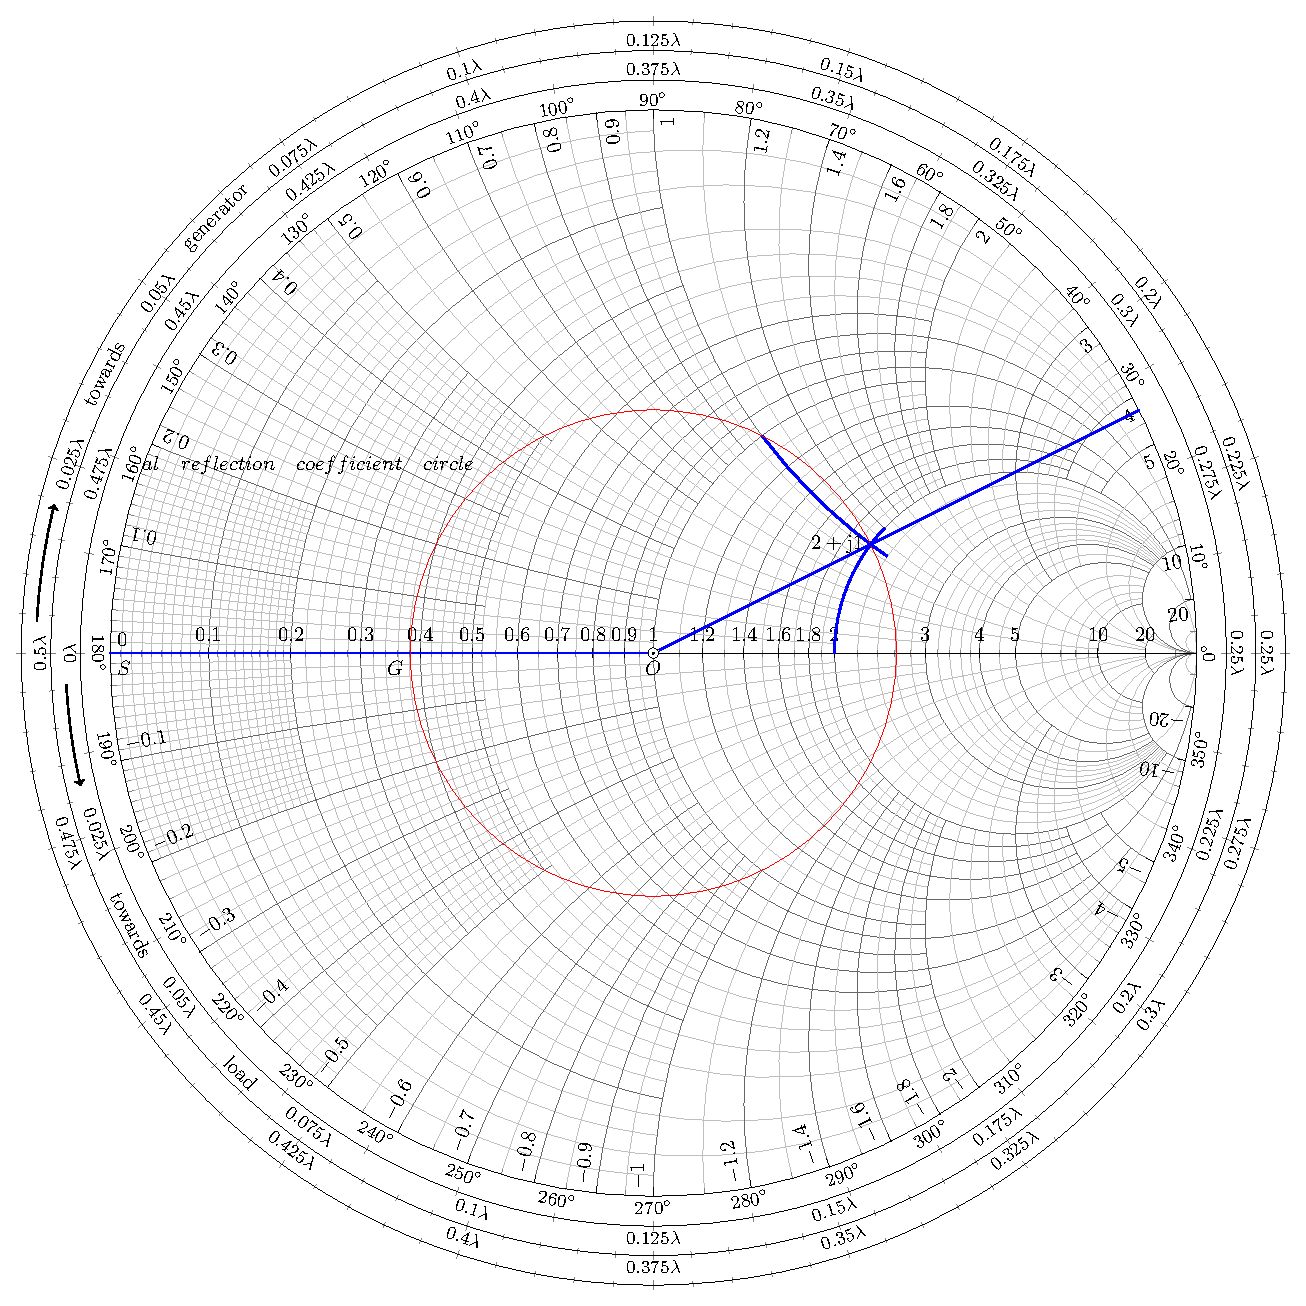
\includegraphics[width=6.5cm]{SCexample7.eps}}
    \only<8>{\includegraphics[width=6.5cm]{SCexample8.eps}}
    \only<9>{\includegraphics[width=6.5cm]{SCexample9.eps}}
    \only<10>{\includegraphics[width=6.5cm]{SCexample10.eps}}
    \only<11>{\includegraphics[width=6.5cm]{SCexample11.eps}}
    
    %\only<1>{\includegraphics[width=6cm]{SCexample1.eps}}
   \end{column}
  \end{columns}
 \end{frame}



\subsection{阻抗匹配}
\begin{frame}{阻抗匹配}

\end{frame}

\subsection{支节匹配器}
\begin{frame}{支节匹配器}

\end{frame}

\subsection{$\lambda/4$ 阻抗变换器}
\begin{frame}{$\lambda/4$ 阻抗变换器}

\end{frame}

\subsection{小反射理论}
\begin{frame}{小反射理论}

\end{frame}

\subsection{二项式(最大平坦特性)多节阻抗变换器}
\begin{frame}{二项式(最大平坦特性)多节阻抗变换器}

\end{frame}

\subsection{切比雪夫(等波纹特性)多节阻抗变换器}
\begin{frame}{切比雪夫(等波纹特性)多节阻抗变换器}

\end{frame}

\subsection{渐变传输线}
\begin{frame}{渐变传输线}

\end{frame}
